\chapter{Architektura systemu, sprzęt i oprogramowanie}
\label{chap:architektura}

\section{Wymagania i koncepcja systemu}
\label{sec:wymagania}

Celem projektowanego systemu jest dostarczenie robotowi mobilnemu informacji o otaczających go obiektach, niezależnie od kierunku w którym się znajdują. Przed przystąpieniem do projektowania systemu należało sformułować wymagania, które system musi spełniać, a następnie na ich podstawie zaprojektowano koncepcje jego działania.
\subsubsection*{Wymagania funkcjonalne}

\begin{itemize}[nosep]
  \item System wykrywa obiekty zadanej klasy w pełnym zakresie
        $360^\circ$ wokół robota.
  \item Dla każdego wykrytego obiektu wyznaczany jest jego kierunek
        (azymut) w układzie współrzędnych robota, klasa oraz pewność detekcji.
  \item Detekcje pochodzące z różnych kamer, dotyczące tego samego obiektu,
        są łączone w jeden wynik.
  \item Każda detekcja opatrzona jest znacznikiem czasu odpowiadającym
        chwili wykonania zdjęcia.
  \item Wyniki są publikowane w środowisku ROS~2, co umożliwia ich
        wykorzystanie przez pozostałe moduły oprogramowania robota.
  \item System umożliwia przeprowadzenie kalibracji kamer oraz wyznaczenie
        ich położenia i orientacji na robocie.
\end{itemize}

\subsubsection*{Wymagania niefunkcjonalne}

\begin{itemize}
  \item Praca w czasie rzeczywistym: częstotliwość detekcji na poziomie
        5--10~klatek na sekundę dla każdej kamery.
  \item Opóźnienie od wykonania zdjęcia do udostępnienia wyniku rzędu
        kilkuset milisekund lub mniejsze.
  \item Niski koszt pojedynczego węzła kamerowego oraz możliwość łatwej
        zmiany liczby kamer.
  \item Minimalne obciążenie komputera nadrzędnego i sieci -- przesyłane
        są wyłącznie wyniki detekcji, a nie obraz.
  \item Bezprzewodowa komunikacja węzłów z komputerem nadrzędnym.
\end{itemize}

\subsubsection*{Koncepcja systemu}

Na podstawie powyższych wymagań przyjęto architekturę rozproszoną,
w której przetwarzanie obrazu odbywa się bezpośrednio na węzłach
kamerowych, a komputer nadrzędny otrzymuje jedynie wyniki detekcji.
Schemat blokowy systemu przedstawiono na rysunku~\ref{fig:schemat-systemu}.

\begin{figure}[htbp]
  \centering
  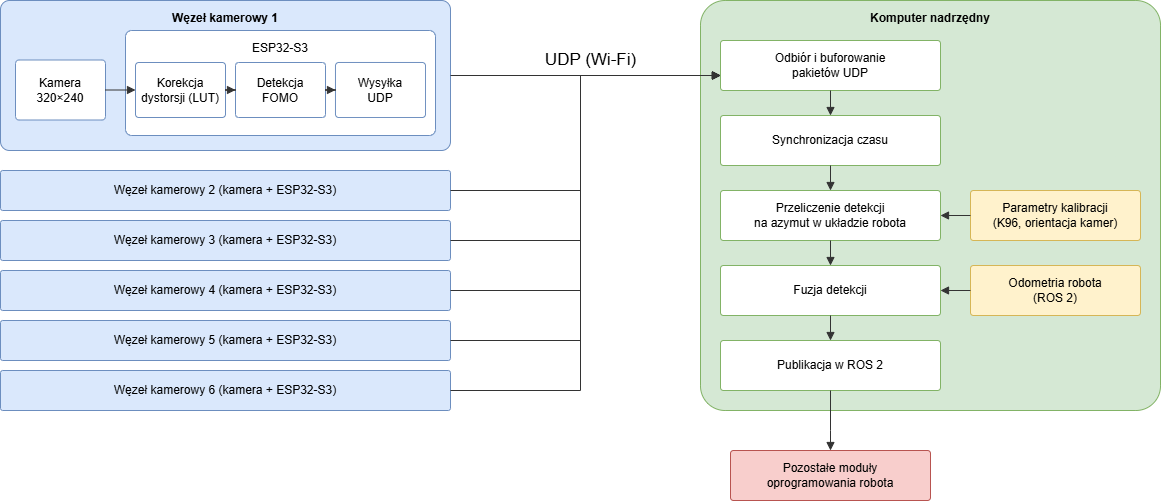
\includegraphics[width=\textwidth]{imgs/schemat_systemu.drawio.png}
  \caption{Schemat blokowy systemu}
  \label{fig:schemat-systemu}
\end{figure}

System składa się z sześciu węzłów kamerowych rozmieszczonych dookoła
robota co $60^\circ$ oraz komputera nadrzędnego. Każdy węzeł zbudowany jest
z mikrokontrolera ESP32-S3 i modułu kamery. Węzły komunikują się
z komputerem przez sieć Wi-Fi z wykorzystaniem protokołu UDP. Obowiązki
poszczególnych elementów podzielono następująco:

\begin{itemize}
  \item \textbf{węzeł kamerowy} -- akwizycja obrazu, korekcja dystorsji,
        inferencja modelu detekcji oraz wysłanie wyniku,
  \item \textbf{komputer nadrzędny} -- odbiór danych ze wszystkich węzłów,
        synchronizacja czasowa, przeliczenie detekcji do układu robota,
        fuzja oraz publikacja wyników w ROS~2.
\end{itemize}

Taki podział wynika z dysproporcji zasobów: mikrokontroler jest w stanie
wykonać inferencję niewielkiej sieci neuronowej, natomiast operacje
wymagające danych ze wszystkich kamer jednocześnie oraz integracja
z ROS~2 realizowane są na komputerze. Dzięki temu na węzłach nie jest
potrzebne środowisko micro-ROS, a ilość przesyłanych danych ogranicza się
do kilkudziesięciu bajtów na klatkę.

% 6 węzłów -> Wi-Fi/UDP -> komputer: fuzja, publikacja w ROS 2



% ===================================================================
% 3.2. Wykorzystany sprzęt  -- wkleić w rozdzial3.tex w miejsce sekcji 3.2
% Miejsca do uzupełnienia oznaczone [UZUPEŁNIĆ: ...] (widoczne w PDF)
% oraz komentarzem % TODO.
% ===================================================================

\section{Wykorzystany sprzęt}
\label{sec:sprzet}

W niniejszym podrozdziale opisano elementy sprzętowe systemu: mikrokontroler
węzła kamerowego, moduł kamery, płytkę węzła wraz z zasilaniem oraz komputer
nadrzędny i sposób jego połączenia z węzłami. Dla mikrokontrolera i kamery
przedstawiono również rozważane alternatywy oraz kryteria wyboru.

% -------------------------------------------------------------------

\subsection{Wybór mikrokontrolera}
\label{subsec:mikrokontroler}
 
Od mikrokontrolera węzła kamerowego wymaga się jednoczesnego spełnienia
kilku warunków: obsługi kamery z równoległym interfejsem danych,
wbudowanej komunikacji Wi-Fi, pamięci wystarczającej do przechowania
bufora klatki i obszaru roboczego modelu (areny) oraz mocy obliczeniowej
pozwalającej na inferencję sieci neuronowej z częstotliwością kilku klatek
na sekundę. Wymagania te spełniają układy SoC z rodziny ESP32 firmy
Espressif, które dodatkowo są tanie i powszechnie dostępne w postaci
gotowych płytek z kamerą.
 
Prace rozpoczęto na module ESP32-CAM (AI-Thinker)~\cite{aithinker_esp32cam}
z układem ESP32-D0WD-V3 i sensorem OV3660. Na tej platformie powstały pierwsze narzędzia do
akwizycji obrazów oraz pierwsze wersje oprogramowania węzła
(podrozdział~\ref{sec:akwizycja-narzedzia}). W trakcie prac ujawniły się
jednak ograniczenia tej platformy, które skłoniły do przejścia na układ
ESP32-S3. Porównanie obu układów zestawiono w tabeli~\ref{tab:esp32-vs-s3}.
 
\begin{table}[htbp]
  \centering
  \caption{Porównanie układów ESP32 (moduł ESP32-CAM) i ESP32-S3 (płytka Goouuu Tech ESP32-S3-CAM)}
  \label{tab:esp32-vs-s3}
  \small
  \begin{tabular}{|l|l|l|}
    \hline
    \textbf{Parametr} & \textbf{ESP32} & \textbf{ESP32-S3} \\
    \hline
    Rdzenie procesora     & 2 $\times$ Xtensa LX6        & 2 $\times$ Xtensa LX7 \\
    Maks. taktowanie      & 240 MHz                      & 240 MHz \\
    Wewnętrzna SRAM       & 520 kB                       & 512 kB \\
    Zewnętrzna PSRAM      & 4 MB (Quad SPI)              & 8 MB (Octal SPI) \\
    Pamięć flash          & 4 MB                         & 16 MB \\
    Instrukcje wektorowe  & brak                         & tak (rozszerzenie PIE) \\
    Optymalizacje ESP-NN  & ogólne (język C)             & asembler z SIMD \\
    Programowanie         & konwerter USB-UART & wbudowane USB \\
    \hline
  \end{tabular}
 
  \vspace{2pt}
  {\footnotesize Źródło: opracowanie własne na podstawie~\cite{espressif_esp32_ds,espressif_esp32s3_ds,espressif_esp32s3_wroom1,aithinker_esp32cam,espressif_espnn}.}
\end{table}
 
Najistotniejszą różnicą są instrukcje wektorowe (SIMD) dostępne w rdzeniach
ESP32-S3 w ramach rozszerzenia PIE (ang. \emph{Processor Instruction
Extensions})~\cite{espressif_esp32s3_trm,espressif_pie_blog}. Biblioteka
ESP-NN wykorzystuje je w implementacjach asemblerowych operacji splotu,
warstw w pełni połączonych i innych operacji sieci neuronowych, natomiast
dla układu ESP32 stosuje jedynie ogólne optymalizacje w języku
C~\cite{espressif_espnn}. Różnicę dobrze ilustrują dane producenta:
model detekcji osób (\emph{person detection}, int8) z areną umieszczoną
w pamięci PSRAM wykonuje się na ESP32-S3 w 54~ms, a na ESP32 w 380~ms,
czyli ok. 7 razy dłużej przy tej samej częstotliwości taktowania
240~MHz~\cite{espressif_espnn}.
Drugim czynnikiem jest pamięć. Arena modelu zajmuje ok. 270~kB i nie mieści
się w wolnej pamięci wewnętrznej, która po uruchomieniu Wi-Fi wynosi ok.
66~kB. Arena musi więc znajdować się w zewnętrznej pamięci PSRAM, a jej
pojemność i szybkość dostępu wpływają na czas wykonania sieci. ESP32-S3
z pamięcią Octal PSRAM taktowaną z częstotliwością 80~MHz oferuje tu
wyraźnie lepsze warunki niż ESP32-CAM.
 
Znaczenie miała również wygoda pracy. Moduł ESP32-CAM nie posiada
wbudowanego złącza USB, a przed każdym wgraniem oprogramowania wymaga
ręcznego zwarcia wyprowadzenia GPIO0 do masy. Płytka z ESP32-S3 programowana
jest bezpośrednio przez USB, co przy sześciu węzłach znacząco upraszcza
aktualizację oprogramowania.
 
% Opcjonalnie: jeżeli zmierzysz czas inferencji własnego modelu FOMO na obu
% układach, dopisz wynik tutaj i odeślij do podrozdziału~\ref{sec:wydajnosc}.
 
Na podstawie powyższych porównań jako platformę węzła kamerowego wybrano
układ ESP32-S3.

% -------------------------------------------------------------------
\subsection{Wybór modułu kamery}
\label{subsec:kamera}


\subsection{Płytka węzła i zasilanie}
\label{subsec:plytka-zasilanie}


\subsection{Komputer nadrzędny i infrastruktura sieciowa}
\label{subsec:komputer-siec}

Odbiór danych z węzłów, fuzja detekcji oraz publikacja wyników w ROS~2
realizowane są na komputerze nadrzędnym. Wykorzystano komputer stacjonarny
z procesorem AMD Ryzen~5 3600 (6~rdzeni, 12~wątków, taktowanie bazowe
3,6~GHz) i 16~GB pamięci RAM, pracujący pod kontrolą systemu Ubuntu 24.04 LTS. Obciążenie obliczeniowe tych zadań jest niewielkie, ponieważ
komputer nie przetwarza obrazu, a jedynie kilka detekcji na klatkę
z każdej kamery. Nie wykorzystuje się w szczególności karty graficznej -
cała inferencja sieci neuronowej odbywa się na węzłach.

Każdy z węzłów przesyła wyniki detekcji do komputera nadrzędnego
z wykorzystaniem protokołu UDP. Węzły i komputer pracują w tej samej
lokalnej sieci, zbudowanej na typowym domowym routerze. Węzły łączą się
z punktem dostępowym routera przez Wi-Fi w paśmie 2,4~GHz (moduł ESP32-S3
obsługuje tylko to pasmo), natomiast komputer jest dołączony do routera
przez Wi-Fi. Adresy IP przydziela
wszystkim urządzeniom serwer DHCP routera. Adres komputera nadrzędnego
i numer portu docelowego (5005) zapisano w konfiguracji oprogramowania
węzłów. Na komputerze program odbiorczy nasłuchuje na tym porcie na
wszystkich interfejsach sieciowych. Nadawcę pakietu rozpoznaje po polu
identyfikatora kamery, a nie po adresie IP. Dzięki temu zmiana adresów
węzłów przy ponownym przydziale DHCP nie wpływa na działanie systemu.

Ilość przesyłanych danych jest bardzo mała. Pojedynczy pakiet zawiera
identyfikator węzła, klasę, współrzędne centroidu, pewność detekcji oraz
znacznik czasu (podrozdział~\ref{sec:pakiet-udp}). Przyjmując rozmiar
pakietu wraz z nagłówkami rzędu 60~B, sześć węzłów pracujących
z częstotliwością ok. 9 klatek na sekundę generuje strumień ok.
$6 \cdot 9 \cdot 60\,\mathrm{B} \approx 3{,}2$~kB/s.
% TODO: podstawić rzeczywisty rozmiar pakietu
Dla porównania przesyłanie surowych klatek QVGA w odcieniach szarości
($320 \cdot 240 = 76{,}8$~kB na klatkę) z tą samą częstotliwością
wymagałoby przepustowości ok. 4,1~MB/s, czyli ok. 33~Mbit/s, co w sieci
Wi-Fi współdzielonej przez sześć urządzeń prowadziłoby do znacznych
opóźnień i utraty danych. Przetwarzanie obrazu na węzłach sprawia więc, że
sieć nie stanowi wąskiego gardła systemu.

\section{Wykorzystane oprogramowanie i narzędzia}
\label{sec:oprogramowanie-narzedzia}

\subsection{Środowisko ESP-IDF i sterownik kamery}
\label{subsec:esp-idf-narzedzie}

\subsection{Edge Impulse, TensorFlow Lite Micro i ESP-NN}
\label{subsec:edge-impulse}

\subsection{Python i OpenCV}
\label{subsec:python-opencv}

\subsection{ROS 2 i RViz}
\label{subsec:ros2-rviz}

\section{Rozmieszczenie kamer}
\label{sec:rozmieszczenie}
% pokrycie 360 stopni, nakładanie pól widzenia, rozdzielczość kątowa komórki FOMO

\section{Budżet opóźnień end-to-end}
\label{sec:budzet-opoznien}
% 171 ms = wiek klatki 61 + LUT 4,5 + DSP 5,3 + sieć 97 + reszta
